%第5章
\chapter{図と色}
\label{ch:pictures}

この章では図の挿入と自動配置の仕方,
そして色について説明したいと思います。



\section{図}
\label{sec:insert-pictures}

他のソフトを使わず,つまり{\LaTeX}だけでも,
例えば{\TikZ}というパッケージを使えば図を描くことができます。
しかし,これは全てコマンドで描かねばならず,
面倒でかつ技術や知識も必要です。

そこで,ExcelやPowerPoint,
または手書きなどで図を用意することが多いと思います。
そうなると,ほとんどの画像がPDFかJPEGで用意されると思うので,
それを想定して書いています
(おそらく他の形式の図にも通用すると思います)。


\subsection{図の挿入}
図の挿入にはgraphicxパッケージを使います。
このgraphicxパッケージは,グラフィック関係全般で使えるパッケージですので,
読み込んでおいて損はないです。
図を挿入したいときは以下のようにします。

\begin{ITeX}
\documentclass[dvipdfmx]{jsarticle}
\usepackage{graphicx}
\begin{document}

\includegraphics[オプション]{図のファイル名}

\end{document}
\end{ITeX}

このdvipdfmxは,ドライバ名で,
{p\TeX},{up\TeX}で標準的に使われるドライバです。
PDF,JPEG,PNG,EPS形式の図を扱うことができます。
他にpdftex,xetex,luatexなどがありますが,
dvipdfmxにしておいて大丈夫です。

図の挿入自体には,
\begin{ITeX}
\includegraphics[オプション]{図のファイル名}
\end{ITeX}
というコマンドを使います。

ファイル名には全角文字は使わず,
半角アルファベットと数字とアンダーバーだけにした方が安全です。
一応,grffileというパッケージを使えば大丈夫みたいですけど。

図のファイルは文書と同じところにおけば大丈夫ですが,
図だけ別で管理したいという場合,
\begin{ITeX}
\graphicspath{{フォルダ1のパス}{フォルダ2のパス}...}
\end{ITeX}
とすれば,フォルダ1,フォルダ2...の中も探してくれます。
また,個々のコマンドでファイル名を絶対パスや相対パスで指定することもできます。
パスの話が分からない人は
第\ref{ch:file-management}章の第\ref{sec:path-and-directory}節を読んでください。

\verb|\includegraphics|につけるオプションには以下のようなものがあります。

\begin{table}[H]
\label{tab:options-of-includegraphics}
\begin{center}
\begin{tabular}{lp{31zw}}
width=長さ &
	幅を指定した長さにします。\tabularnewline
height=長さ &
	高さを指定した長さにします。\tabularnewline
totalheight=長さ &
	高さ+深さが指定できます。
	図を回転したときに便利です。\tabularnewline
keepaspectratio &
	widthとheightを両方指定したとき,
	縦横比を変えずに指定した幅,高さに図を入れます。\tabularnewline
scale=倍率 &
	画像のサイズが倍率倍されます。\tabularnewline
clip &
	描画領域の外側を描かないという指定です。
	周囲の文書が侵食されるのを防ぐために指定します。
	これは指定しておくのが安全です。\tabularnewline
trim = $x_1 \ y_1 \ x_2 \ y_2$ &
	左 $x_1$,下 $y_1$,右 $x_2$,上 $y_2$ だけ図を切り詰めます。
	単位は1/72インチです。\tabularnewline
viewpoint= $x_1 \ y_1 \ x_2 \ y_2$ &
	元の画像の左下の角を原点として,
	左下の角を $(x_1, y_1)$,右上の角を $(x_2, y_2)$ とした
	長方形の領域を切り出します。
	こちらも単位は1/72インチです。\tabularnewline
angle=角度(単位は度) &
	画像を指定した角度だけ回転します。\tabularnewline
origin=位置 &
	画像の回転の中心を指定します。
	この位置には,lrctbBがあり,それぞれ
	左,右,中央,上,下,ベースラインを表しています。
	この位置の中から2つまで選んで指定します。
	また,[x=2mm, y=3mm]のように
	座標で指定することもできます\tabularnewline
units=6.2832 &
	回転の角度の単位を,度からラジアンに変更します。
\end{tabular}
\end{center}
\end{table}

図を入れたいところが何かしらの環境の中だったりすると
エラーを吐くことがあります。
そのときは,minipage環境を作ってその中で
\verb|\includegraphics|をすれば大抵の場合は大丈夫です。
このminipage環境は横幅を引数に取り,
\begin{ITeX}
\begin{minipage}{0.4\hsize}
\includegraphics{picture.pdf}
\end{minipage}
\end{ITeX}
などのようにして使います。
この\verb|\hsize|はページの横幅を設定しているコマンドですので,
\verb|0.4\hsize|は全ページ幅の4割を表しています。


\subsection{図の自動配置}
\label{subsec:pictures-auto-distribution}
図の自動配置にはfigure環境を使います。
また,図にはキャプションとラベルをつけることができます。
例えば以下のように,

\begin{ITeX}
\begin{figure}
\includegraphics[width=10cm]{parabola.pdf}
\caption{関数$y = x^2$のグラフ}
\label{fig:parabolagraph}
\end{figure}
\end{ITeX}

とすれば,
下にキャプションのついたグラフが
自動的に配置されて出力されます。
この図を参照するときは,
\verb|図\ref{fig:parabolagraph}において...| のようにして
2回出力すればよいです。
この\verb|\label|や\verb|\ref|,
2回実行する意味については
相互参照やリンクを扱う第\ref{ch:reference-contents-link}章で詳しく扱います。

このfigure環境には以下のようなオプションがあります。

\begin{table}[H]
\label{tab:options-of-figure}
\begin{center}
\begin{tabular}{lp{40zw}}
t & ページ上部に図を出力します。\tabularnewline
b & ページ下部に図を出力します。\tabularnewline
p & 単独ページに図を出力します。\tabularnewline
h & 出来ればその位置に図を出力します。\tabularnewline
H & 必ずその位置に図を出力します(floatパッケージが必要)。
\end{tabular}
\end{center}
\end{table}

なお,このオプションはデフォルトでは[tbp]になっています。

図の番号は自動的に「図1」,「図2」,...のように付きます。
これを「Fig.1」のようにしたければ,
jsarticle,jsbookなら
\begin{ITeX}
\documentclass[english]{jsarticle}
\end{ITeX}
のように,englishオプションを付けます。
それ以外のドキュメントクラスでは,
\begin{ITeX}
\renewcommand{\figurename}{Fig.}
\end{ITeX}
のようにプリアンブルに書いておきます。

\verb|\caption{図の説明}|は図の説明を出力するコマンドですが,
\verb|\listoffigures|とすれば,
その説明を使った図目次をその位置に出力することができます。
説明が長いときなどは,オプションに短い説明をつけ,
それを図目次に出力することもできます。
図目次については,目次を扱う章もご覧ください。


\subsection{図を左右に配置する}
2つの図を上下でなく左右に配置したいときもあると思います。
ここではそのやり方を扱います。

関連のない2つの図を左右に配置するときは,
figure環境の中にminipage環境を作って,

\begin{ITeX}
\begin{figure}
\begin{center}
\begin{minipage}{0.4\columnwidth}
    \begin{center}
    \includegraphics[width=\columnwidth]{figure1.pdf}
    \end{center}
    \caption{左側}
    \label{fig:left}
\end{minipage}
\begin{minipage}{0.4\columnwidth}
    \begin{center}
    \includegraphics[width=\columnwidth]{figure2.pdf}
    \end{center}
    \caption{右側(左と連関無し)}
    \label{fig:right}
\end{minipage}
\end{center}
\end{figure}
\end{ITeX}

のようにすれば,次のようになります。

\begin{figure}[H]
\begin{center}
\begin{minipage}{0.4\columnwidth}
	\begin{center}
	
\framebox[\columnwidth]{図}
	\end{center}
	\caption{左側}
	\label{fig:left}
\end{minipage}
\begin{minipage}{0.4\columnwidth}
	\begin{center}
	
\framebox[\columnwidth]{図}
	\end{center}
	\caption{右側(左と連関無し)}
	\label{fig:right}
\end{minipage}
\end{center}
\end{figure}

なお,\verb|\columnwidth|は本文の幅を表します。
minipage中ではminipageの幅が\verb|\columnwidth|になるので
上のようにしています。
また,minipage自身の幅は好きに指定してください。

関連のある2つの図を左右に配置したいときは,
subcaptionパッケージを利用します。
まずはプリアンブルに\verb|\usepackage{subcaption}|と書いてください。
これの使い方は,上とほぼ同じで,
minipageをsubfigureに置き換えて,

\begin{ITeX}
\begin{figure}
\begin{center}
\begin{subfigure}{0.4\columnwidth}
    \begin{center}
    \includegraphics[width=\columnwidth]{figure1.pdf}
    \end{center}
    \caption{左側}
    \label{fig:left}
\end{subfigure}
\begin{subfigure}{0.4\columnwidth}
    \begin{center}
    \includegraphics[width=\columnwidth]{figure2.pdf}
    \end{center}
    \caption{右側(左と連関無し)}
    \label{fig:right}
\end{subfigure}
\end{center}
\caption{左右両方}
\label{fig:left-and-right}
\end{figure}
\end{ITeX}

とします。
この出力は次のようになります。

\begin{figure}[H]
\begin{center}
\begin{subfigure}{0.4\columnwidth}
    \begin{center}
	
\framebox[\columnwidth]{図}
    \end{center}
    \caption{左側}
    \label{fig:left_sub}
\end{subfigure}
\begin{subfigure}{0.4\columnwidth}
    \begin{center}
	
\framebox[\columnwidth]{図}
    \end{center}
    \caption{右側(左と連関無し)}
    \label{fig:right_sub}
\end{subfigure}
\end{center}
\caption{左右両方}
\end{figure}

左右の図がくっついて見づらいときは,
\verb|\end{subfigure}|と\verb|\begin{subfigure}|の間に
適当に\verb|\hspace|でも入れてください。



\section{図の回り込み配置}
\label{sec:wrapfig}

\begin{wrapfigure}{r}{10zw}
\vspace*{-\intextsep}
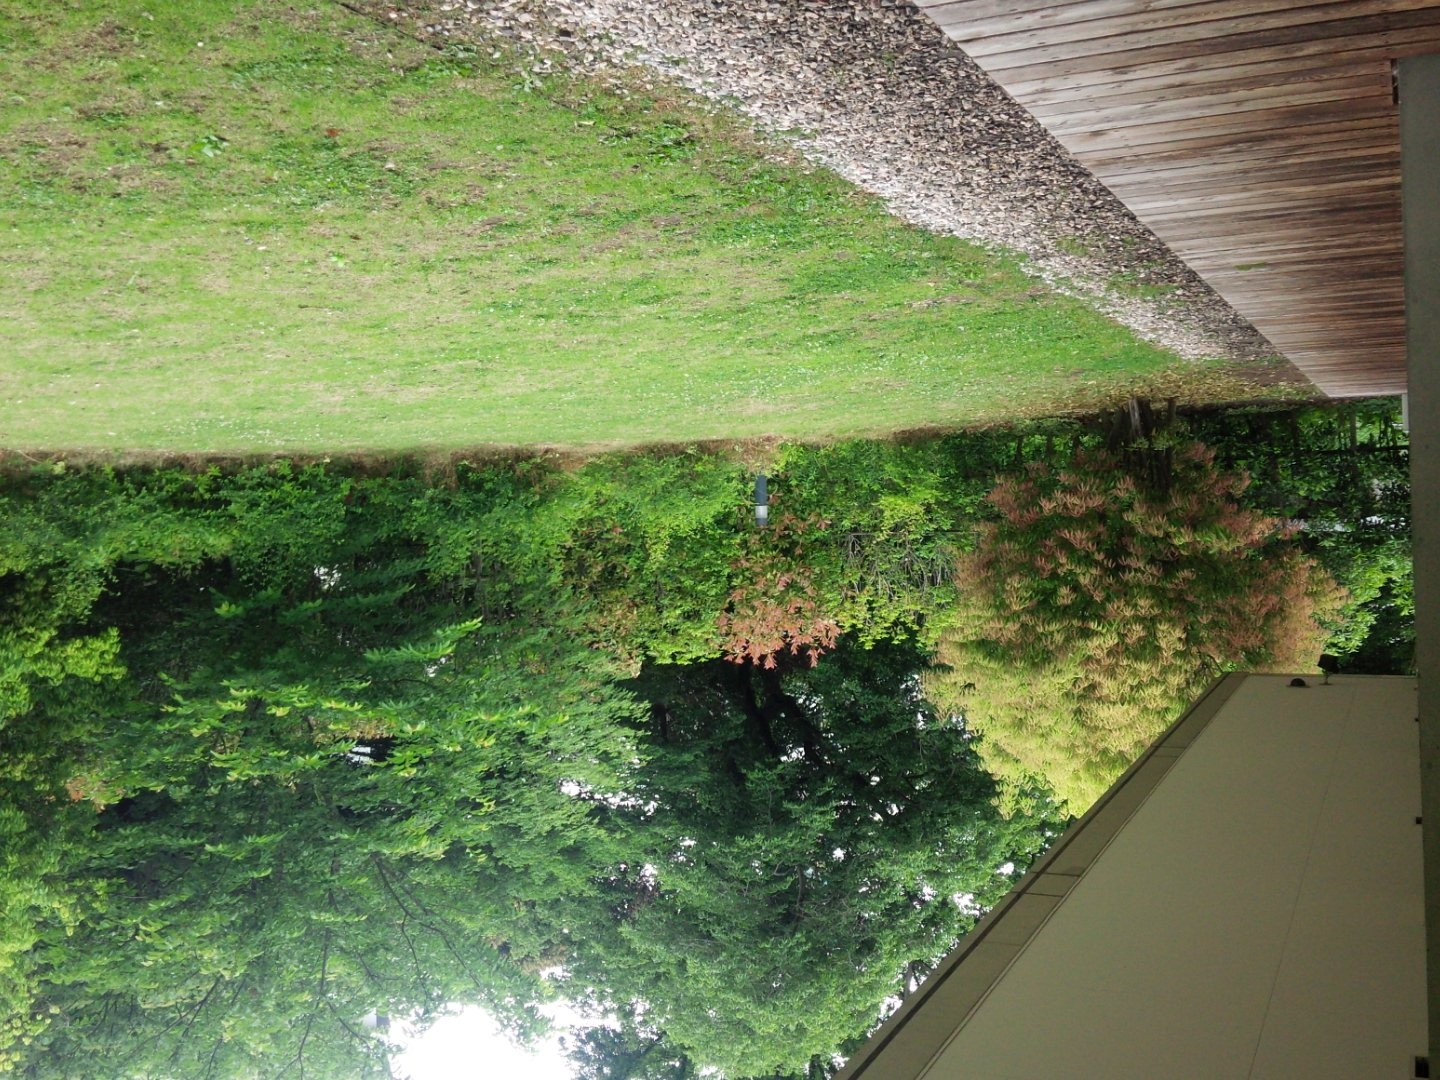
\includegraphics[clip, width=10zw, angle=180]{figures_for_pictures/wakan.jpg}
\end{wrapfigure}

図を文書の右とか左に配置したいときもあるかと思います。
例えばこのように。
そんなときは,wrapfigパッケージのwrapfigure環境が便利です。

使い方について説明します。
まずはプリアンブルに
\begin{ITeX}
\usepackage{wrapfig}
\end{ITeX}
と書いてください。
例えば,上のように図を回り込ませたいときは,
\begin{ITeX}
\begin{wrapfigure}{r}{10zw}
\vspace*{-\intextsep}
\includegraphics[width=10zw]{huukei.jpg}
\end{wrapfigure}
\end{ITeX}
のように書きます。
\verb|\begin{document}|の1つ目の引数に位置(lかr),
2つ目の引数にその幅を指定します。
オプションで行数も指定できます。
ただ,これは自動で計算してくれるので特に指定する必要はありません。
まとめると,以下のように使うということです。
\begin{ITeX}
\begin{wrapfigure}[行数]{位置(lかr)}{幅}
\end{ITeX}

上に示した例に\verb|\vspace*{-intextsep}|とありますが,
これはデフォルトで入る縦方向のスペース分上に戻す,という操作をしています。
これを入れるとちょうどいいって話ですね。

なお,wrapfigには表の回り込み配置用にwraptable環境も用意されているので,
必要ならば使ってみて下さい。
また,注意ですが,
このwrapfigure環境は箇条書き系の環境
(難しいことを言うと,ボックスを生成するもの)
と相性が悪いので,
併用は避けてください。
箇条書きと併用したいときはmawarikomiパッケージを使ってみて下さい。
また,floatパッケージを使う場合は,
floatパッケージの後に読み込んでください。



\section{色}
\label{sec:colors}

色の表し方には,RGBとCMYKの2通りがあります。
RGB(Red, Green, Blue)は
ディスプレイの色に使われる表し方で,
赤・緑・青の3色を,0~255の256段階に分け,
その値で色を表します。
CMYK(Cyan, Magenta, Yellow, blacK)は
印刷物に使われる表し方です。

このRGBとCMYKは互換性がなく,
変換がかなり大変らしいのですが,
僕はよくわからないですし,
変換をしなくてもある程度似た色で印刷されるみたいなので,
この話は割愛します。

色を使うときはxcolorパッケージを使います。
まずはプリアンブル(\verb|\documentclass|と\verb|\begin{document}|の間)に
\begin{ITeX}
\usepackage{xcolor}
\end{ITeX}
と書いてください。

字の色を変えることが多いと思うので,そのやり方を説明します。

グレースケールを指定するときは,
\begin{ITeX}
{\color[gray]{0.5} 文字}
\textcolor[gray]{0.5}{文字}
\end{ITeX}
のようにします。
この数値は,黒を0,白を1として,0~1で指定します。

CMYKを指定するときは,
\begin{ITeX}
{\color[cmyk]{0.75, 0.64, 0, 1} 文字}
\textcolor[cmyk]{0.75, 0.64, 0, 1}{文字}
\end{ITeX}
のようにします。

RGBについては,3通りの表し方があります。
各RGB値を255で割った値を使って,
\begin{ITeX}
{\color[rgb]{0.75, 1, 0} 文字}
\textcolor[rgb]{0.75, 1, 0}{文字}
\end{ITeX}
のようにするのが一般的なようですが,
RGB値をそのまま使って,
\begin{ITeX}
{\color[RGB]{120, 255, 0} 文字}
\textcolor[RGB]{120, 255, 0}{文字}
\end{ITeX}
のようにもできます。
また,HTMLにおける色の指定法を用いて,
\begin{ITeX}
{\color[HTML]{10A3FF} 文字}
\textcolor[HTML]{10A3FF}{文字}
\end{ITeX}
のようにすることもできます。

いちいち色を数値で指定するのは面倒ですので,
いくつかの色はもともと定義されており,
その名前を書くだけで使えます。
また,xcolorパッケージにdvipsnamesオプションを付けると,
もっと多くの色名を使うことができます。

しかし,これだけでは欲しい色が手に入らない,
という場合もあると思います。
そのときは,次のようにして色を定義します。
\begin{ITeX}
\definecolor[gray]{x}
\definecolor[rgb]{r, g, b}
\definecolor[cmyk]{c, m, y, k}
\end{ITeX}
RGBについては,文字色の変更のときと同様,
オプションをRGBやHTMLにして,
それに従った記法で定義することもできます。

元々ある色名や定義した色名を使って,
次のように色を指定することもできます。
\begin{ITeX}
{\color{色名} 文字}
\textcolor{色名}{文字}
\end{ITeX}
なお,\verb|\color|コマンドは,
適用範囲を\verb|{}|で囲まないと
それ以降全ての文字の色が変わってしまうので注意が必要です。

ページの色を変えるには,
\begin{ITeX}
\pagecolor{色名}
\end{ITeX}
とします。
それ以降のページは全てその色になるので,
白に戻すには\verb|\pagecolor{white}|とします。

文字の背景に色を付けたいときは,
\begin{ITeX}
\colorbox{色名}{文字}
\end{ITeX}
とします。
なお,色名はオプションと数値でも指定できます。
\colorbox{lightcyan}{例えばこんな風に}

これに枠を付けたいときは,
\begin{ITeX}
\fcolorbox{枠色}{背景色}{文字}
\end{ITeX}
とします。
\fcolorbox{orange}{lightcyan}{わくわく}

